% Chapter 1 of the Thesis Template File
\chapter{INTRODUCTION AND  BACKGROUND}

%This is the opening paragraph to my thesis which explains in general terms the concepts and hypothesis which will be used in my thesis.

%This section will cover the basic and general concepts of my thesis.  This will be a high level approach to the problem and to the proposed solution.  In addition, this section gives a general background to the project

%This chapter has 4 sub-sections.  1)  Introduction to SDRs, 2) Introduction to GNURadio and 3) Introduction to the current ISU radiometer and finally the 4th is the Related Works section

\section{Introduction}
The goal of this thesis is to explore the use of a software defined radio that can function as well as or better than current radiometers.  In addition, we aimed to develop a radiometer that is more flexible than most radiometers and still maintain the accuracy and stability of a traditional radiometers if not exceed these specifications.  A secondary goal was to use off the shelf components and components that are generally more accessible and often less expensive.  This would allow radiometers to be more accessible to a wider scope of researchers in this field.  And finally a tertiary goal was to ensure that the system as a whole is fairly easy to use.  This ties to our secondary goal of making radiometers more accessible to a wider range of researchers and research topics.

This thesis looks to explore the following questions: (1) Can we use an off the shelf SDR along with GNURadio to recreate a radiometer in software that is easy to use and cost effective?  (2) If so, what performance can we get from the system?  (3) What benefits do we gain (if any) from using a SDR from a more traditional radiometer? The results of this research and experimentation are the subject of this thesis.


\subsection{Software Defined Radio Radiometer}

Software defined radios consist of both hardware and software that allow it to perform the operations that is required.  A software defined radio used for radiometer applications is identical to a software defined radio used for, as an example, a 802.11b radio with one major difference.  Since we do need to amplify the signal more than what most communication applications require, we do have more powerful or additional LNAs to boost this signal.  In addition, since the first LNA plays a major role in the overall system noise and this system noise does affect performance of the radiometer, the selection of this LNA is important.  However, all other components are the same components used in other applications.

A software defined radio radiometer behaves analogous to a more traditional radiometer and thus can be used in the same type of applications as a traditional radiometer.  This includes applications such as radio astronomy and can also be used in Earth Science applications such as soil moisture and ocean salinity[\cite{Ruf}].  A software defined radio radiometer can also allow for new applications to be introduced as well.  Since we have moved the majority of the hardware to software this allows us to further shrink the size and weight of the radiometer.  This can allow for radiometers to be used in other applications such as Unmanned Aerial Vehicles (UAVs) for scanning things such as ocean salinity remotely[\cite{McIntyre}].  

We will now introduce the three major components that make up a software defined radio radiometer.  

%\textbf{N200 SDR}
\subsubsection{N200 Software Defined Radio} 
The key component for a software defined radio radiometer is of course the software defined radio or SDR.  The equipment that was selected for researching into this topic was the Ettus Research Group N200 SDR.  This SDR uses daughter boards as the RF front end to the SDR and up to two daughter boards may be installed into a N200.  This is an important consideration as one of the requirements is to be able to look at both the V-Pol and the H-Pol signal coming from the antenna.  This allows us to correlate the signal and other signal analysis can also be done.  Another important reason the N200 was selected was due to the fact that it can handle up to 50 MHz of bandwidth to the computer.  This means that it is very possible to have two receive cards that can stream up to 25 MHz bandwidth each.  

The N200 utilizes a flexible architecture for a variety of RF interface systems based on the frequency range desired and if receive and/or transmission is needed.  These daughter boards directly receive the RF signal and then outputs the analog I and Q signals that are then sampled by the N200 A/D converter for reception or receives the I and Q values from the N200 D/A converter for transmission. 

{\begin{figure}[h!tb] 
\centering
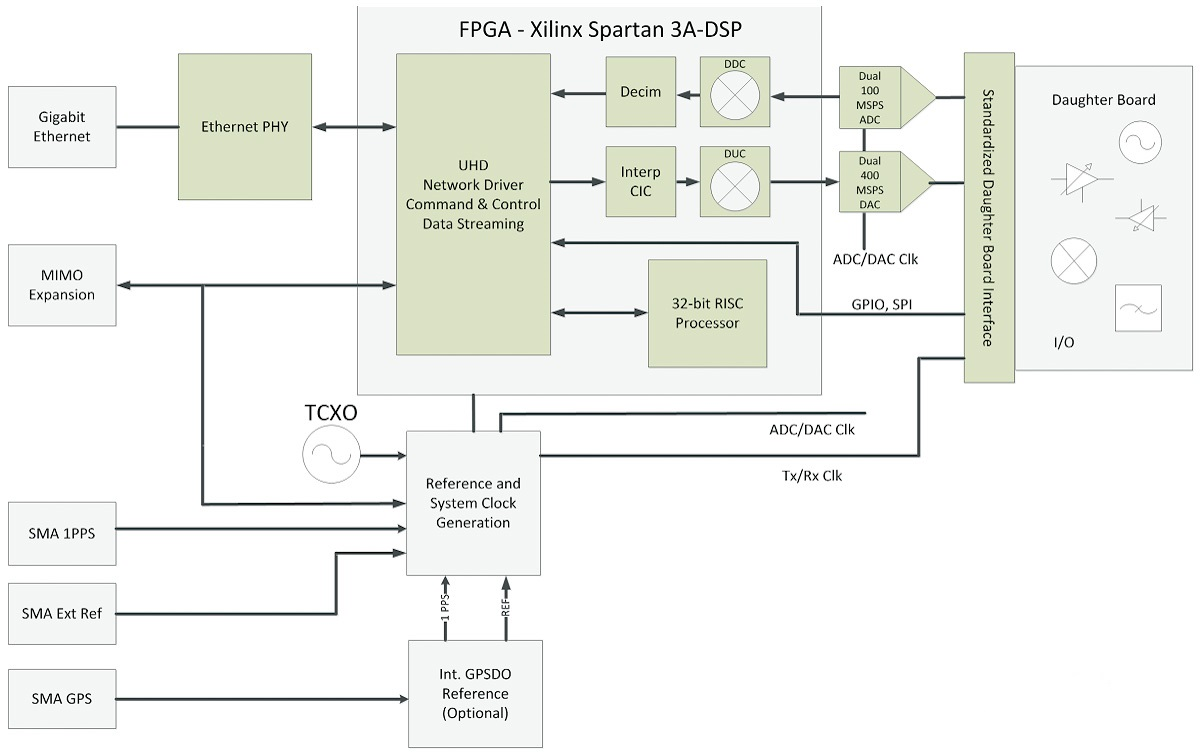
\includegraphics[width=14cm]{Images/n200_block_edited}
\isucaption{Block diagram of the N200 SDR}
\label{N200_block}
\end{figure}
}

The daughter board selected was the DBSRX2 card.  This card is a receive only card that operates between 800 MHz and 2.4 GHz and would thus work in the 1.4 GHz band we are interested in.  The DBSRX2 also has built in amplification that is adjustable through software.

\subsubsection{GNURadio Software}

For the software portion of the radio, we settled to use GNURadio, an open source software package that is well supported by the community and by the Ettus Research Group and the N200 SDR.  GNURadio also comes with what is known as GNURadio Companion or GRC.  This program provides us with a GUI interface and allows for the drag and drop of blocks that represent certain functions that can be used with the SDR.  GNURadio and GRC use Python as it's main scripting language and GNURadio uses C++ code for directly accessing the hardware.  The hardware interface for the N200 is provided by Ettus as well.  They provide drivers that allow GNURadio to talk to their hardware.  Like GNURadio, these drivers are also available to all platforms.  In addition, Ettus has released these drivers to the open source community.

GNURadio has been ported to several platforms including Windows, Mac OS X and Linux.  Linux is by far the most popular platform to work on and most of this thesis research was done within the Linux environment.  Testing was also done though with a MacBook Pro running OS X 10.9.  The OS X implementation is fairly well supported and is installed through MacPorts.  

Through GNURadio, we can now write code that will take the data given to us from the SDR and manipulate the signal as we need to mimic a radiometer.  The power detection, filtering and recording of this data is all done through GNURadio.  This also means that we are shifting more of the computational power done on the signal from the FPGA to a computer running GNURadio.  There are ways to change this behavior and upload code directly to the FPGA.  However for this thesis it was easier to debug and work with GNURadio by keeping the processing on the desktop computer.  It does however mean that the host computer must be powerful enough to handle the signal and specifically the large bandwidth that we wish to send to it.  

\subsection{RF Front End}
The RF front end plays a critical role in the radiometer as the LNAs used in the front end has a large impact on the system noise generated by the radiometer itself.  A traditional radiometer utilizes both amplification through the LNAs and also includes filtering to the desired bandwidth.  A SDR radiometer does not require the filters as we are able to create these in software, however the amplification stages need to remain.  

{\begin{figure}[h!tb] 
\centering
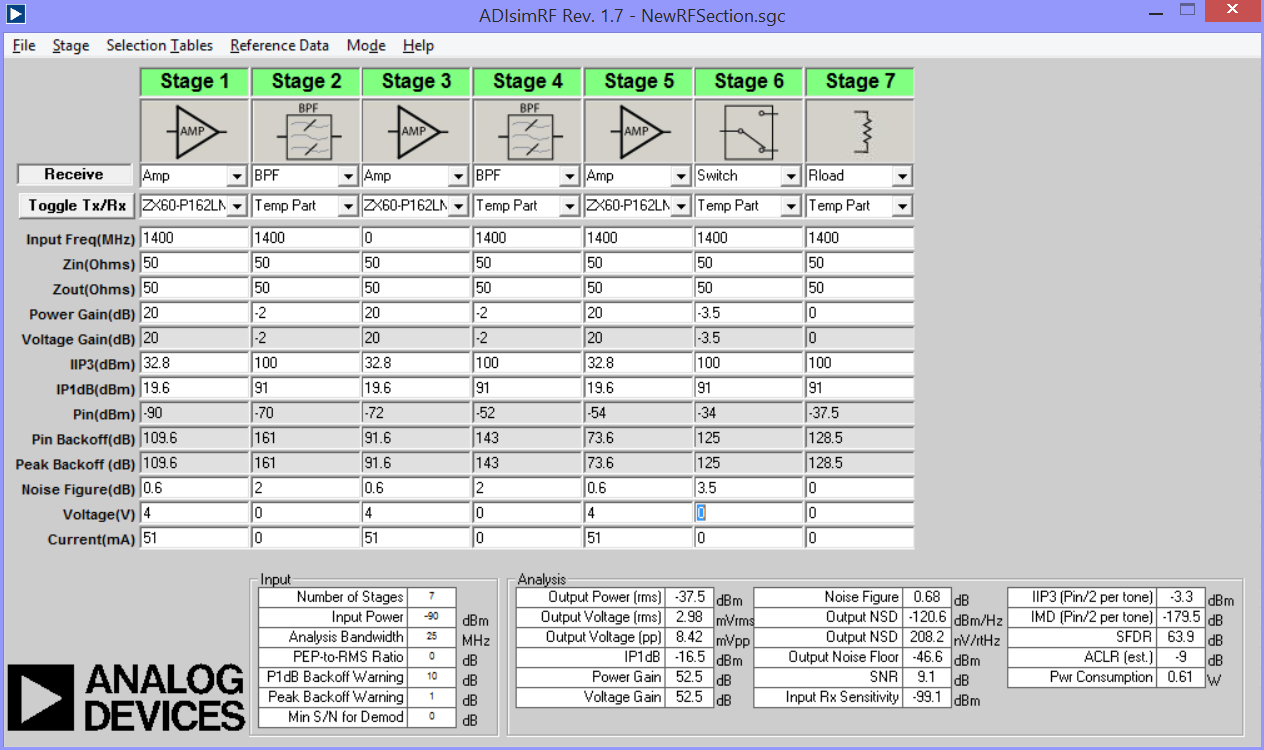
\includegraphics[width=0.8\linewidth]{Images/RF_Front_end.png}
\isucaption{The ADISIMRF program used to verify the design of the RF Front End}
\label{ISU_Rad}
\end{figure}
}
A typical RF front end uses a 3 stage Low Noise Amplifier (LNA) to amplifier the noise while keeping the noise contributed to the system as low as possible.  As with any radiometer, the first LNA is the most critical as it contributes the most to the overall system noise temperature.  For this reason a LNA that did not have a large gain but had a very low noise figure was chosen. The second and third LNA has higher gain values at the cost of a higher noise figure, although not by much.  However, since they are further down the chain, they do not contribute as much to the total system noise.  The reason for this is further explained in chapter 3. 

\section{Background}
\textbf{Software Defined Radios} 
Software Defined Radios (SDRs) have been used for a variety of applications, but their primary application has been in the area of communications.  They appeal to applications where being able to change a modulation scheme or filter on the fly is desirable.  In these areas, SDRs often outperform a traditional hardware only radio with their ability to rapidly change their operations by simply changing their software.  Early SDRs were expensive due to the high costs in the analog to digital converters (ADCs) needed and in the high speed Field Programmable Gate Arrays (FPGA) used.  In recent years however, the cost of SDRs have decreased due to the cost of these key components decreasing in cost as well.  Even though the cost has gone down, the performance of many SDRs have increased.  This has lead to new applications for SDRs being developed and using SDRs in new and different ways.

The basic concept behind a SDR is that it will digitize the RF signal as soon as possible.  Once digitized, it can now be evaluated by a computer, FPGA, or a dedicated System on Chip (SoC).  A canonical software defined radio architecture is one that consists of a power supply, antenna, multi-band RF converter, and a single chip that contains the needed processing and memory to carry out the radio functions in software [\cite{Mitola1995}]. This allows us to extract certain hardware functions, such as filtering, into the digital domain which can then be manipulated by software.  Since software is now manipulating the signal, we can rapidly change what functions we execute on the signal by changing the software.  This gives SDRs a high amount of flexibility as various components that are normally done in hardware can now be done in software and can be changed by simply uploading new software or firmware to the system.  This also gives us a benefit in cost as certain components are no longer needed and changes done in software do not require additional hardware to be added or to be swapped out.

\textbf{Radiometers}  
Radiometers are radio receivers that simply listen to and record the amount of power received.  However, the power received is not a coherent signal, instead it is the amount of noise the radiometer sees.  Radiometers, at the basic level, listen to noise that is generated naturally from a source.  These sources can vary and the applications vary as well.  Some examples of radiometer applications have been in evaluating soil moisture content, ocean salinity levels and celestial objects[\cite{ulaby2014}].

The amount of noise that is generated is due to the thermal agitation of the charge carriers, usually the electrons, which is directly correlated to the physical temperature of the source[\cite{Nyquist1928thermal}].  This correlation is done as a noise temperature.  Various objects can emit this noise and the intensity will vary on various parameters and on what the source is.  One source that has current research at Iowa State University is in detecting soil moisture.  Various soil types can be observed including sandy types of soil[\cite{Liu}], The brighter or warmer the noise temperature is, the more RF noise that has been received which correlates to a drier soil.  The less RF noise power received, the cooler the noise temperature and this indicates wetter soil area. Radiometers such as these are already in service on satellites such as the Soil Moisture and Ocean Salinity (SMOS) satellite launched by the European Space Agency (ESA) and are used by scientists to monitor the Earth's soil moisture and ocean salinity[[\cite{McMullan}][\cite{Hardy}].  

A traditional radiometer uses several Low Noise Amplifiers (LNAs), filters and power is often measured using a square law detector.  Even though we are measuring noise, we want to measure the right noise and we want the noise generated by the radiometer hardware itself to be as low as possible.  In other words, we are really listening to the noise being generated from an outside source.  Additional noise in the system is impossible to eliminate, however we can take steps to reduce it as much as possible.  In addition, we can calculate what this noise is and take steps to account for it in our measurements.  However, this means that stability is another factor within the radiometer.  If the noise generated within the radiometer is constantly changing, this makes it difficult to account for this additional noise.  There are steps we can take to work with this though.  A traditional method often used is the Dicke radiometer which switches between the measurement of the antenna and a known source[\cite{Dicke}].  By referencing this known source the Dicke radiometer can calibrate and account for any drift due to variations in the system.  Another method is to use highly stable components and keep them stable during the operation of the radiometer.  For LNAs, temperature directly effects the overall gain from the LNA.  In some radiometer applications we can control the temperature which allows us to keep the LNAs stable during the operation.  Stability will be discussed in greater detail later in this thesis.

Additional improvements to radiometers have also been done by digitizing parts of the radiometer.  The most common method for doing this is by digitizing the analog output of the square-law detector and sending that to a computer or processing unit to analyze the data[\cite{Bremer}].  While this does allow for easier computation and storage of the information, it does not alleviate the needs to maintain stability or reduce possible additional noise of the system since this data is digitized after the RF signal chain.

\textbf{A more modern Radiometer}  
Iowa State University currently owns a 1.4 GHz, dual polarization, correlating radiometer.  This radiometer is currently in use by Dr. Brian Hornbuckle and his research team.  However, in recent years the radiometers digital circuitry has suffered from various issues which has made it unusable.  Part of the driving force behind this research in this thesis is to determine new methods that can be used to rebuild this radiometer.

The ISU Radiometer was built at the University of Michigan and put into service at ISU in 2006.  The ISU radiometer is unique in that it is one of the few direct sampling radiometers in use\cite{Erbas}.  This radiometer takes the RF signal, amplifies and filters the signal, and then sends it directly to an analog to digital converter.  At the time the ISU radiometer was built, an A/D that could sample accurately at 1.4 GHz were expensive and hard to come by due to the fact that Nyquist's theorem states that we must sample at least two times the frequency.  However, the ISU radiometer does not sample at 2.8 GHz or above, instead it samples at 1.4 GHz.  The reason the ISU radiometer can do this is due to the fact that a radiometer is generally only interested in the power of the incoming signal.  This means that we are not interested in recreating the entire signal and therefore we can under-sample the signal.  The A/D data is then sent to a Field Programmable Gate Array (FPGA) which then processes the data.  The ISU radiometer is also a correlating radiometer, which means that it looks at both the vertical polarization (V-Pol) and the horizontal polarization (H-Pol) and then correlates this information[\cite{Fischman2001}].  

\section{Related Works}
As mentioned before, software defined radios have been used in a number of applications.  While as far as the author has determined, this is the first application of using an off the shelf software defined radio for a radiometer in remote sensing for soil moisture measurements, there has been similar applications done.  The closest application that has been found is with radio astronomy.  Radiometers used in radio astronomy is nothing new and has been used for quite some time[\cite{Ohm}]. by There are many similarities between radio astronomy and remote sensing of the ground.  Both are using a radiometer to listen to a source of interest.  In radio astronomy the basic principal is that a "hot" source such as a star will produce more noise than the cooler background of space.  In remote sensing we are looking at the overall change of the source to determine it's characteristics.  In both cases we are measuring the total power of the noise and based on that information we can determine some properties of the source we are looking at.

\subsection{Radio Astronomy Examples}
The Shirleys Bay Radio Astronomy Consortium (SBRAC) located in Smiths Falls, Ontario is currently using a USRP software defined radio in conjunction with GNURadio.  SBRAC has successfully used this configuration to obtain radio astronomy data by looking at the hydrogen line at 1420.4058 MHz [\cite{Leech2007}].  The person in charge of this facility, Marcus Leech, contributed software to the GNURadio specifically for radio astronomy applications.  It was this software branch that was used as the base for the GNURadio program that was used in this thesis.  Marcus Leech continue to contribute to the GNURadio community and continues to provide support for these functions as well[\cite{Leech}].

Another example of a software defined radio used as a radiometer is from students at the University of Illinois and Grand Valley State University that built a software defined radio to listen to emissions from Jupiter[\cite{Behnke}].  This software defined radio was built using an Analog Devices AD9460 and a Xilinx Spartan-3E-500 FPGA to build the SDR itself.  A RF front end was also built to filter and amplify the signal coming into the SDR.  Finally, this group also used GNURadio to interface to and talk to the SDR and used both Python and wxGUI to build a working interface.  The students reported that the SDR radiometer worked very well and was able to do so at a fairly low price point.

It should be noted that much of the related works found worked with using a radiometer for astronomy or for looking at the sky.  For the ISU radiometer however, we are looking at the ground and we are using the radiometer for soil moisture instead of measuring stars and other points of interest in the sky.  While the fundamentals is the same for either radiometer, some adjustments need to be made due to the fact that a radiometer looking at the sky often sees a "cool" brightness temperature whereas a radiometer looking at the ground sees a much "warmer" brightness temperature.  This is due to the albedo of the Earth and the fact that it has a much warmer noise temperature then what you find with radio astronomy[\cite{Tiuri}].
\subsection{Other Digital Radiometers}

A digital radiometer is not a new concept.  Early radiometers would often digitize the analog voltage information from the square-law detector and then send that information to a computer for storage or analysis.  

A pre-cursor to a software defined radio, some radiometers would also digitize the incoming RF signal, but under-sample this information.  Since only power is the information desired this was acceptable.  However, these radiometers did often use the same components you might find in a software defined radio such as an A/D converter and FPGA.  These components however were used in different ways.

One reason why these devices were used differently from a SDR was due to cost.  Most radiometer operations happen at 1.4 GHz or above.  A/D converters at these higher frequencies become more expensive and harder to obtain.  In recent years however, these costs have come down.

The major difference between other digital radiometers and what is discussed in this thesis is that we retain both phase and magnitude information and instead mimics a traditional radiometer in software by summing and squaring the I and Q values and then running this information through a low-pass IIR filter.  By retaining this information, we can perform a more in-dept analysis of the signal coming into the radiometer which allows for greater agility in the system.